\documentclass{beamer}
\usetheme{Frankfurt}
\usecolortheme{seahorse}
\setbeamercolor{background canvas}{bg=}

\usepackage[utf8]{inputenc}

\usepackage{sourcecodepro}
\usepackage[pdf]{graphviz}

\usepackage{tikz}
\usepackage{xcolor}
\usepackage{soul}
\definecolor{code}{rgb}{0.95, 0.95, 0.95}
\sethlcolor{code}
\newcommand{\code}[1]{\colorbox{code}{\texttt{\footnotesize #1}}}

\usepackage{csquotes}
\newcommand{\q}[1]{\enquote{#1}}

\usepackage{listings}
\usepackage{ifthen}
\tikzstyle{highlighter} = [
  lime,
  line width = \baselineskip-0.3em,
]
\newcounter{highlight}[page]
\newcommand{\tikzhighlightanchor}[1]{\ensuremath{\vcenter{\hbox{\tikz[remember picture, overlay]{\coordinate (#1 highlight \arabic{highlight});}}}}}
\newcommand{\bh}[0]{\stepcounter{highlight}\tikzhighlightanchor{begin}}
\newcommand{\eh}[0]{\tikzhighlightanchor{end}}
\AtBeginShipout{\AtBeginShipoutUpperLeft{
  \ifthenelse{\value{highlight} > 0}{
    \tikz[remember picture, overlay]{
      \foreach \stroke in {1,...,\arabic{highlight}}
        \draw[highlighter] (begin highlight \stroke) -- (end highlight \stroke);
    }
  }{}
}}
\lstdefinestyle{j}{
  keywordstyle=\textbf,
  commentstyle=\textit,
  basicstyle=\ttfamily\scriptsize,
  tabsize=4,
  numbers=left,
  escapechar=`,
}
\newcommand{\IncludeCode}[2]{
  \lstinputlisting[style=j, language=java, caption={#2}]{#1}
}

\usepackage{cite}

\AtBeginSection[]{
  \begin{frame}
    \begin{beamercolorbox}[sep=0.5em, center, shadow=true]{title}
      \usebeamerfont{title}\insertsectionhead\par
    \end{beamercolorbox}
  \end{frame}
}

\title{Data flow analysis for Uranus applications}
\author{Chan Kwan Yin}

\begin{document}

\frame{\titlepage}

\begin{frame}
  \frametitle{Outline}
  \tableofcontents
\end{frame}

\section{Background}

\begin{frame}
  \frametitle{SGX Enclaves}
  \begin{columns}
    \begin{column}{0.5\textwidth}
      \begin{itemize}
        \item Servers outsourced to third-party cloud providers
        \item Threat model: Adversaries with privileged access to OS, BIOS or hardware
        \item Enclave protects both code and memory from these adversaries
      \end{itemize}
    \end{column}
    \begin{column}{0.5\textwidth}
      \digraph[scale=0.35]{EnclaveExample}{
        compound = true;
        %
        subgraph cluster_enclave {
          label = "enclave";
          color = "red";
          %
          secret_key [label = "secret key"];
          decrypted [label = "decrypted input"];
          decryption [shape = "box";]
          anonymization [shape = "box"];
          secret_key -> decryption;
          decryption -> decrypted;
          decrypted -> anonymization;
        }
        %
        encrypted_input [label = "encrypted input"];
        output [label = "output"];
        encrypted_input -> decryption;
        anonymization -> output;
        %
        adversary [label = "Adversary", shape="diamond"];
        adversary -> decrypted [lhead = cluster_enclave, color = "red", dir = "none"];
        adversary -> output [dir = "none", color = "forestgreen"];
        encrypted_input -> adversary [dir = "none", color = "forestgreen"];
      }
    \end{column}
  \end{columns}
\end{frame}

\begin{frame}
  \frametitle{Uranus \cite{uranus}}
  \begin{itemize}
    \item OpenJDK fork that supports Intel SGX
    \item Methods marked as \code{@JECall} enters enclaves until return
    \item Methods marked as \code{@JOCall} exits enclaves until return
    \item Useful for integration with libraries like Hadoop and Spark
    \item Question: Where should \code{@JECall} and \code{@JOCall} be placed?
    \item Question: Is code in these libraries safe as enclave code?
  \end{itemize}
\end{frame}

\begin{frame}[t]
  \frametitle{The problem: Performance/Security Tradeoff}
  \begin{itemize}
    \item More code outside enclave:
      \begin{itemize}
        \item Increased risk of leaking protected data
        \item Some leaks may come from unexpected side channels
      \end{itemize}
    \item More code into enclave:
      \begin{itemize}
        \item Limited EPC (Enclave Page Cache)
          \begin{itemize}
            \item Up to 100 MB of EPC
            \item Out of memory $\implies$ extremely slow swap
            \item JVM applications especially memory-greedy
          \end{itemize}
        \item Principle of Least Privilege
          \begin{itemize}
            \item Vulnerabilities in enclave code bypass enclave protection
            \item Vulnerabilities in code outside must only use specific entry points
            \item Reduce attack surface
          \end{itemize}
      \end{itemize}
  \end{itemize}
\end{frame}

\begin{frame}[fragile]
  \frametitle{The solution}
  \begin{itemize}
    \item Select the minimum cover of sensitive data
    \item \textit{enclavlow} \footnote{coined from the words "enclave" and "flow"}:
      an information flow analysis tool
    \item Sources of sensitive data marked with \code{sourceMarker}
    \item Anonymization marked with \code{sinkMarker}
    \item Identity functions; expected to be optimized them away by JIT
  \end{itemize}

  \begin{lstlisting}[style=j, language=java]
  @JECall
  static int process(byte[] encrypted) {
    byte sum = 0;
    byte[] password = `\bh`sourceMarker`\eh`(new byte[]{1, 2, 3, 4, 5, 6});
    byte[] decrypted = decrypt(password, encrypted);
    for(byte b : decrypted) sum ^= b;
    return `\bh`sinkMarker`\eh`(sum);
  }
  \end{lstlisting}
\end{frame}

\begin{frame}
  \frametitle{Threat model}
  \begin{itemize}
    \item Adversary has no read/write access to enclave code and memory
    \item Adversary has arbitrary access to any system resource,
      \emph{including} non-enclave Java and JVM memory
    \item The actual adversary also has access to hardware resources,
      including sensor modules, system clock, etc.
    \item These resources can be used to implement side channel attacks,
      which are system-dependent, environment-dependent and architecture-dependent
    \item Example: Timing attack based on CPU branch prediction optimization
    \item Our adversary model excludes these side channel attacks
  \end{itemize}
\end{frame}

\begin{frame}
  \frametitle{Changes on Uranus model}
  \begin{itemize}
    \item Applications are expected to run on a Uranus-based JVM.
    \item Some behaviour disallowed by Uranus assumed permissible under explicit indication
    \item Assignment to objects outside enclaves
      \begin{itemize}
        \item Reads are assumed copied into enclave
        \item Writes are assumed always leaking
      \end{itemize}
    \item Assignment to static fields
      \begin{itemize}
        \item Reads are cloned into enclave
        \item Writing enclave-local data may not be expected behaviour
        \item Assumed immediate leak
      \end{itemize}
    \item Expected to integrate into Uranus for compile-time checking/optimization
  \end{itemize}
\end{frame}

\section{Approach}
\begin{frame}[fragile]
  \frametitle{Intuition: Trivial ways of leaking data}
  \begin{lstlisting}[language=java, style=j]
    static int outside; // static variables stored outside enclave
    @JOCall void println(int x);

    int secret() {
      return sourceMarker(123456);
    }

    @JECall int foo() {
      `\bh`store`\eh` = secret(); // assigning to static field
      `\bh`println`\eh`(secret()); // passing secret to a JOCall
      `\bh`return`\eh` secret(); // returning secret out of a JECall
    }
  \end{lstlisting}
\end{frame}

\begin{frame}[fragile]
  \frametitle{Intuition: Non-trivial ways of leaking data}
  \begin{itemize}
    \item Assigning to an outside-enclave object:
      \begin{lstlisting}[language=java, style=j, gobble=8, tabsize=2]
        @JECall void x(Box box) {
          `\bh`box.`\eh`value = secret();
        }
      \end{lstlisting}
    \item Leaking control flow into variables:
      \begin{lstlisting}[language=java, style=j, gobble=8, tabsize=2]
        `\bh`if`\eh`(secret() >= 3) outside++;
        `\bh`for`\eh`(int i=0; i < secret(); i++) outside++;
      \end{lstlisting}
    \item Implicit exceptions:\\
      \begin{lstlisting}[language=java, style=j, gobble=8, tabsize=2]
        int[] array = new int[3];
        array`\bh`[`\eh`secret()`\bh`]`\eh` = 1;
      \end{lstlisting}
    \item Transitive application of above
  \end{itemize}
\end{frame}

\begin{frame}
  \frametitle{Flow graph}
  \begin{itemize}
    \item Analysis framework: Soot \cite{sootsurvivor}
    \item Each readable/writable data entry as a node
    \item $(x, y) \in E \implies$ placement of $y$ outside enclave
      reduces indistinguishability of $x$
    \item $(x, y), (y, z) \in E$: transitive
    \item $(x, y), (x, z) \in E$: Leaking \emph{either} $y$ \emph{or} $z$ distinguishes $x$
    \item No way to represent requirement of \emph{both} $y$ \emph{and} $z$
  \end{itemize}
\end{frame}

\begin{frame}
  \frametitle{Procedure}
  \begin{enumerate}
    \item Each method is analyzed independently as a Local Flow Graph (LFG)
    \item LFG contracted into subgraph of only "public" nodes called Contract Flow Graph (CFG)
    \item CFGs merged together into Aggregate Flow Graph (AFG),
  \end{enumerate}
\end{frame}

\begin{frame}
  \frametitle{Local flow graph}
  \begin{itemize}
    \item Analyze each method independently using Soot's \code{ForwardBranchedFlowAnalysis}
    \item Soot calls the \code{flowThrough} method for each 3AC (jimple) statement
    \item Each \code{flowThrough} maps the state in the previous step to a new state
    \item For branching statements, each branch has a its own state
    \item When flows converge, soot calls the \code{merge} method to map two states into a new one
  \end{itemize}
\end{frame}

\begin{frame}[fragile]
  \frametitle{Implementing \code{flowThrough} for assignment operations}
  \begin{itemize}
    \item For each type of value, define
      \begin{itemize}
        \item rvalue nodes
        \item lvalue nodes for assignment
        \item and lvalue nodes for deletion
      \end{itemize}
    \item Pseudocode:
      \begin{lstlisting}[style=j, gobble=8, tabsize=2, basicstyle=\ttfamily\tiny]
        Algorithm assign($left = $right):
          for each lvalues($left, FLAG_DELETION) as $node:
            delete (*, $node) from flow graph
          for each lvalues($left) as $leftNode:
            add (CTRL, $leftNode) to flow graph
            for each rvalues($right) as $rightNode:
              add ($rightNode, $leftNode) to flow graph // intuitive
          for each lvalues($right) as $leftNode:
            for each rvalues($left) as $rightNode:
              add ($rightNode.*, $leftNode.*) to flow graph // field projection
      \end{lstlisting}
  \end{itemize}
\end{frame}

\begin{frame}
  \frametitle{Global nodes}
  \begin{itemize}
    \item Static node
      \begin{itemize}
        \item All reads use Uranus cache
        \item Writes are assumed immediate leak
      \end{itemize}
    \item Explicit source/sink
      \begin{itemize}
        \item Explicit sink is cosmetic
      \end{itemize}
  \end{itemize}
\end{frame}

\begin{frame}
  \frametitle{Method signature nodes}
  \begin{itemize}
    \item Parameter nodes
      \begin{itemize}
        \item Supports both read and write
      \end{itemize}
    \item This node
      \begin{itemize}
        \item just an alternative parameter
      \end{itemize}
    \item Return node
    \item Throw node
      \begin{itemize}
        \item just an alternative return path
      \end{itemize}
  \end{itemize}
\end{frame}

\begin{frame}
  \frametitle{The CTRL node}
  \begin{itemize}
    \item Tracks what data affect the current flow
    \item Each branched block has its CTRL node
    \item $(x, \text{CTRL}) \in E \implies \exists$ predicate $p$ such that
      the branch represented by CTRL executes if and only if $p(x)$
    \item $(\text{CTRL}_1, \text{CTRL}_2) \in E$ when
      $\text{CTRL}_2$ is a subbranch of $\text{CTRL}_1$
    \item $(\text{CTRL}, y) \in E \implies$ leaking $y$ may distinguish whether CTRL was run
    \item Merging states: select Lowest Common Ancestor
  \end{itemize}
\end{frame}

\begin{frame}
  \frametitle{Other nodes}
  \begin{itemize}
    \item Local variables
      \begin{itemize}
        \item Including temp values created by Jimple
      \end{itemize}
    \item Method calls
      \begin{itemize}
        \item Blackbox proxies to signature nodes
      \end{itemize}
  \end{itemize}
\end{frame}

\begin{frame}
  \frametitle{Contraction and aggregation}
  \begin{itemize}
    \item At each return point, track flow from "public" nodes into the following nodes:
      \begin{itemize}
        \item \code{this}
        \item \code{static}
        \item explicit sink
        \item parameters
        \item method calls (proxy nodes)
      \end{itemize}
    \item At aggregation, connect each proxy node to the actual implementation
      \begin{itemize}
        \item Polymorphism?
      \end{itemize}
  \end{itemize}
\end{frame}

\section{Case study}

\begin{frame}[fragile, t]
  \frametitle{Case study: Branching (tableswitch)}
  \begin{columns}[t]
    \begin{column}{0.5\textwidth}
      \begin{lstlisting}[style=j, language=java, gobble=6, tabsize=2, basicstyle=\ttfamily\tiny]
        public static int switchMux(int x,
            int a, int b, int c, int d) {
          switch (x) {
            case 16: return a;
            case 17: return b;
            case 18: return c;
            default: return d;
          }
        }
      \end{lstlisting}
      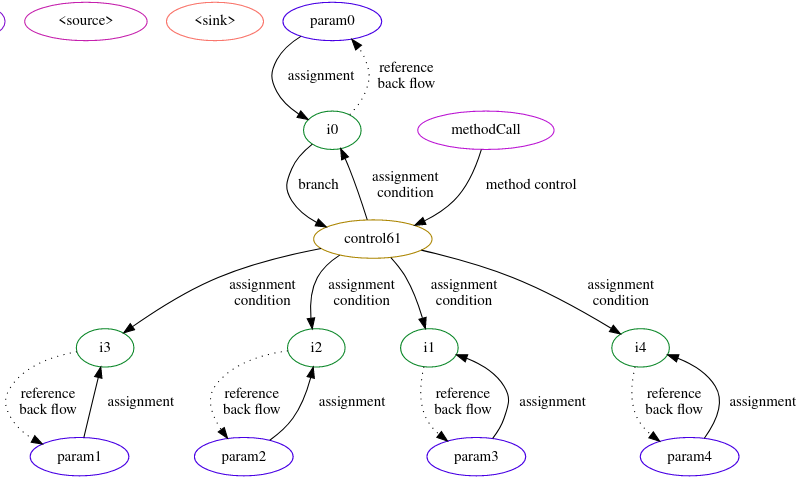
\includegraphics[scale=0.28]{screenshot20201217125744.png}
    \end{column}
    \begin{column}{0.5\textwidth}
      \begin{lstlisting}[style=j, gobble=6, tabsize=2, basicstyle=\ttfamily\tiny, numbers=none]
        public static int switchMux
            (int, int, int, int, int) {
          int i0, i1, i2, i3, i4;
          i0 := @parameter0: int;
          i3 := @parameter1: int;
          i2 := @parameter2: int;
          i1 := @parameter3: int;
          i4 := @parameter4: int;
          tableswitch(i0) {
              case 16: goto label1;
              case 17: goto label2;
              case 18: goto label3;
              default: goto label4; };
        label1: return i3;
        label2: return i2;
        label3: return i1;
        label4: return i4; }
      \end{lstlisting}
    \end{column}
  \end{columns}
\end{frame}

\begin{frame}[fragile, t]
  \frametitle{Case study: Loops}
  \begin{columns}[t]
    \begin{column}{0.4\textwidth}
      \begin{lstlisting}[style=j, language=java, gobble=6, tabsize=2, basicstyle=\ttfamily\tiny]
        public static int loopInc(int i) {
          int a = 0;
          for (int j = 0; j < i; j++) {
              a += j;
          }
          return a;
        }

      \end{lstlisting}
      \begin{lstlisting}[style=j, gobble=6, tabsize=2, basicstyle=\ttfamily\tiny]
        public static int loopInc(int) {
          int i0, i1, i2;
          i0 := @parameter0: int;
          i1 = 0;
          i2 = 0;
        label1:
          if i2 >= i0 goto label2;
          i1 = i1 + i2;
          i2 = i2 + 1;
          goto label1;
        label2: return i1; }
      \end{lstlisting}
    \end{column}
    \begin{column}{0.6\textwidth}
      {\tiny.} % columns hack
      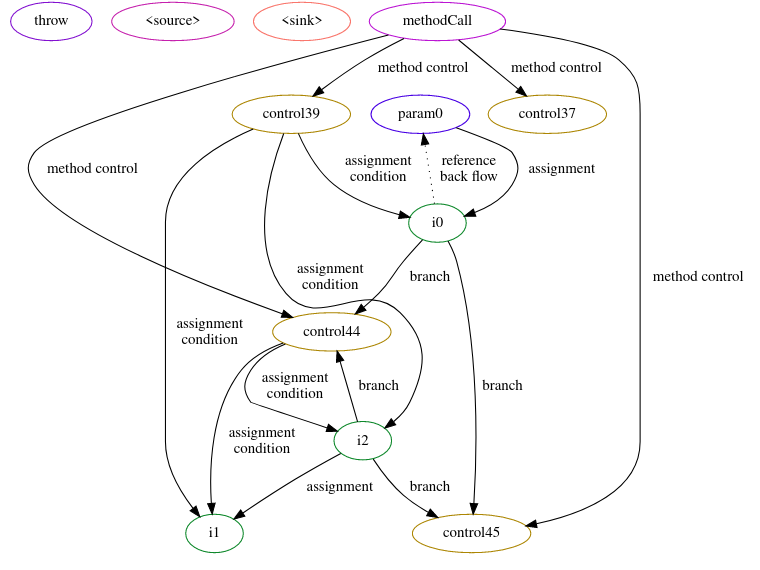
\includegraphics[scale=0.25]{screenshot20201217140733.png}
    \end{column}
  \end{columns}
\end{frame}

\begin{frame}[fragile]
  \frametitle{AFG: Full Example}
  \begin{columns}
    \begin{column}{0.5\textwidth}
      \begin{lstlisting}[language=java, style=j, gobble=6, tabsize=2, basicstyle=\ttfamily\tiny]
      @JECall
      int getSum(byte[] enc) {
        byte[] dec = parse(enc);
        return sinkMarker(computeSum(dec)); }

      byte[] parse(byte[] enc) {
        byte[] otp = sourceMarker(PRIVATE_KEY);
        byte[] result = new byte[enc.length];
        for(int i = 0; i < buf.length; i++)
          result[i] = enc[i] ^ otp[i];
        return result; }

      int computeSum(byte[] bytes) {
        int result = 0;
        for(byte b : bytes) result += (int) result;
        return result; }
      \end{lstlisting}
    \end{column}
    \begin{column}{0.5\textwidth}
      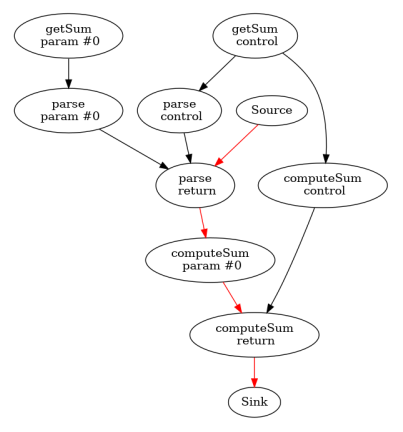
\includegraphics[scale=0.4]{screenshot20201217010535.png}
    \end{column}
  \end{columns}
\end{frame}

\section{Limitations}
\begin{frame}
  \frametitle{False negatives: implicit exceptions}
  \begin{itemize}
    \item Conditional runtime errors leaks data
      \begin{itemize}
        \item \code{NullPointerException}
        \item \code{IndexOutOfBoundsException}
      \end{itemize}
    \item Too sensitive to raise an exception path for every array access and object access
    \item Good practice: exceptions should be caught at enclave boundary anyway!
    \item Solutions usually achieved at the language level,
      e.g. \code{@NonNull}, \code{@Size}
    \item Do not reinvent the wheel
  \end{itemize}
\end{frame}

\begin{frame}[fragile]
  \frametitle{False positives: identical branches}
  \begin{itemize}
    \item This does not leak \code{secret}
      (assuming \code{doSomething*()} do not leak control flow)
      \begin{lstlisting}[style=j, language=java, gobble=6, tabsize=2]
        boolean foo() {
          int secret = getSecret();
          if(secret > 1) {
            doSomething();
            return false;
          } else {
            doSomethingElse();
            return false;
          }
        }
      \end{lstlisting}
    \item Suggested fix: factorize common code out of branches (good code style)
  \end{itemize}
\end{frame}

\begin{frame}[fragile]
  \frametitle{False positives: self-anonymization}
  \begin{itemize}
    \item This does not leak \code{secret}
      (assuming \code{doSomethingWith(int)} does not leak)
      \begin{lstlisting}[style=j, language=java, gobble=6, tabsize=2]
        int foo(int a) {
          int secret = getSecret();
          a += secret;
          doSomethingWith(a);
          a -= secret;
          return a;
        }
      \end{lstlisting}
    \item Suggested fix: create a clone of \code{a}
    \item Immutability paradigms?
      \begin{itemize}
        \item We are considering the \emph{compiled binary} layer,
          so functional programming languages do not help
      \end{itemize}
  \end{itemize}
\end{frame}

\begin{frame}
  \frametitle{Tackling polymorphism}
  \begin{itemize}
    \item Computing all combinations of instance classes requires exponential time.
    \item Solution: union of CFGs of all possible subclasses
      \begin{itemize}
        \item Iago attacks is still possible if code is used elsewhere in enclave
        \item Therefore all subclasses, not only those through call analysis, are considered
      \end{itemize}
  \end{itemize}
\end{frame}

\begin{frame}
  \frametitle{Tackling JNI calls}
  \begin{itemize}
    \item Assumptions:
      \begin{itemize}
        \item parameters are independent
        \item return value is the output
        \item control flow is not leaked
      \end{itemize}
    \item False negative example: \code{System.arraycopy}
    \item Uranus turns system calls into \code{OCall}s,
      which leak control flow.
  \end{itemize}
\end{frame}

\section{Conclusion}
\begin{frame}
  \begin{itemize}
    \item Assist with decisions on performance/security tradeoff
    \item Incorporated into Uranus
    \item Room for improvement on false negative cases
    \item Integration with source level analysis
  \end{itemize}
\end{frame}

\begin{frame}
  \frametitle{References}
  \scriptsize
  \bibliographystyle{acm}
  \bibliography{cite}
\end{frame}

\end{document}
